\newcommand{\comp}{\TT{comp()}\xspace}
\chapter{\IFRU{Указатели на функции}{Pointers to functions}}
\label{sec:pointerstofunctions}

\index{\CLanguageElements!\Pointers}
\IFRU{Указатель на функцию, в целом, как и любой другой указатель, просто адрес указывающий на начало функции 
в сегменте кода.}
{Pointer to function, as any other pointer, is just an address of function beginning in its code segment.}

\index{Callbacks}
\IFRU{Это применяется часто в т.н. callback-ах}{It is often used in callbacks}
\footnote{\url{http://en.wikipedia.org/wiki/Callback_(computer_science)}}.

\IFRU{Известные примеры:}{Well-known examples are:}

\begin{itemize}
\item
\qsort\footnote{\url{http://en.wikipedia.org/wiki/Qsort_(C_standard_library)}},
{\TT{atexit()}}\footnote{\url{http://www.opengroup.org/onlinepubs/009695399/functions/atexit.html}} \IFRU{из стандартной библиотеки Си}{from the standard C library}; 
\item
\IFRU{сигналы в *NIX ОС}{signals in *NIX OS}\footnote{\url{http://en.wikipedia.org/wiki/Signal.h}};
\item
\IFRU{запуск тредов}{thread starting}: \TT{CreateThread()} (win32), \TT{pthread\_create()} (POSIX);
\item
\IFRU{множество функций win32, например}{a lot of win32 functions, e.g.} \TT{EnumChildWindows()}\footnote{\url{http://msdn.microsoft.com/en-us/library/ms633494(VS.85).aspx}}.
\end{itemize}

\index{\CStandardLibrary!qsort()}
\IFRU{Итак, функция \qsort это реализация алгоритма ``быстрой сортировки''. 
Функция может сортировать что угодно, 
любые типы данных, но при условии, что вы имеете функцию сравнения двух элементов данных и 
\qsort может вызывать её.}
{So, \qsort function is a \CCpp standard library quicksort implementation. The functions is able to sort
anything, any types of data, if you have a function for two elements comparison and \qsort is able
to call it.}

\IFRU{Эта функция сравнения может определяться так:}{The comparison function can be defined as:}

\begin{lstlisting}
int (*compare)(const void *, const void *)
\end{lstlisting}

\IFRU{Воспользуемся немного модифицированным примером, который я нашел вот}
{Let's use slightly modified example I found} \href{http://cplus.about.com/od/learningc/ss/pointers2_8.htm}
{\IFRU{здесь}{here}}:

\lstinputlisting[numbers=left,label=qsort_c_src]{patterns/18_pointers_to_functions/17_1.c}

\section{MSVC}

\IFRU{Компилируем в MSVC 2010 (я убрал некоторые части для краткости) с опцией \Ox}
{Let's compile it in MSVC 2010 (I omitted some parts for the sake of brevity) with \Ox option}:

\lstinputlisting[caption=\Optimizing MSVC 2010: /Ox /GS- /MD]{patterns/18_pointers_to_functions/17_2_msvc_Ox.asm}

\IFRU{Ничего особо удивительного здесь мы не видим. В качестве четвертого аргумента, 
в \qsort просто передается адрес метки \TT{\_comp}, где собственно и располагается функция \comp.}
{Nothing surprising so far.
As a fourth argument, an address of label \TT{\_comp} is passed, that is just a place
where function \comp located.}

\IFRU{Как \qsort вызывает её?}{How \qsort calling it?}

\index{Windows!MSVCR80.DLL}
\IFRU{Посмотрим в MSVCR80.DLL (эта DLL куда в MSVC вынесены функции из стандартных библиотек Си):}
{Let's take a look into this function located in MSVCR80.DLL (a MSVC DLL module with C standard library functions):}

\lstinputlisting[caption=MSVCR80.DLL]{patterns/18_pointers_to_functions/17_3_MSVCR.lst}

\TT{comp}\EMDASH{}\IFRU{это четвертый аргумент функции. 
Здесь просто передается управление по адресу указанному в \TT{comp}. 
Перед этим подготавливается два аргумента для функции \comp. 
Далее, проверяется результат её выполнения.}
{is fourth function argument.
Here the control is just passed to the address in the \TT{comp} argument.
Before it, two arguments prepared for \comp. Its result is checked after its execution.}

\IFRU{Вот почему использование указателей на функции ~--- это опасно. 
Во-первых, если вызвать \qsort с неправильным указателем на функцию, 
то \qsort, дойдя до этого вызова, может передать управление неизвестно куда, 
процесс упадет, и эту ошибку можно будет найти не сразу.}
{That's why it is dangerous to use pointers to functions.
First of all, if you call \qsort with incorrect pointer to function, \qsort may pass control
to incorrect point, a process may crash and this bug will be hard to find.}

\IFRU{Во-вторых, типизация callback-функции должна строго соблюдаться, 
вызов не той функции с не теми аргументами не того типа, 
может привести к плачевным результатам, 
хотя падение процесса это и не проблема, проблема ~--- это найти ошибку, ведь компилятор 
на стадии компиляции может вас и не предупредить о потенциальных неприятностях.}
{Second reason is the callback function types must comply strictly, calling wrong function
with wrong arguments of wrong types may lead to serious problems, however, process crashing is not a 
big problem~---big problem is to determine a reason of crashing~---because compiler may be 
silent about potential trouble while compiling.}

\subsection{MSVC + \olly}
\index{\olly}

\IFRU{Загрузим наш пример в \olly и установим брякпойнт на ф-ции \comp}
{Let's load our example into \olly and set breakpoint on \comp function}.

\IFRU{Как значения сравниваются, мы можем увидеть во время самого первого вызова \comp}
{How values are compared we can see at the very first \comp call}: \figname \ref{fig:qsort_olly1}.
\RU{Для удобства, }\olly \IFRU{показывает сравниваемые значения в окне под окном кода}
{shows compared values in the window under code window, for convenience}.
\IFRU{Мы можем так же увидеть что}{We can also see that the} \ac{SP} \IFRU{указывает на}{pointing to} 
\ac{RA} \IFRU{где находится место в ф-ции}{where the place in} 
\qsort \EN{function is }(\IFRU{на самом деле, находится в}{actually located in} \TT{MSVCR100.DLL}).

\IFRU{Трассируя}{By tracing} (F8) \IFRU{до инструкции}{until} \TT{RETN} 
\IFRU{и нажав F8 еще один раз, мы возвращаемся в ф-цию}{instruction, and pressing F8 one more time, 
we returning into} \qsort\EN{ function}: \figname \ref{fig:qsort_olly2}.
\IFRU{Это был вызов ф-ции сравнения}{That was a call to comparison function}.

\IFRU{Вот также скриншот момента второго вызова ф-ции}{Here is also screenshot of the moment of the 
second call of} \comp\EMDASH{}\IFRU{теперь сравниваемые значения другие}
{now values to be compared are different}:
\figname \ref{fig:qsort_olly3}.

\begin{figure}[H]
\centering
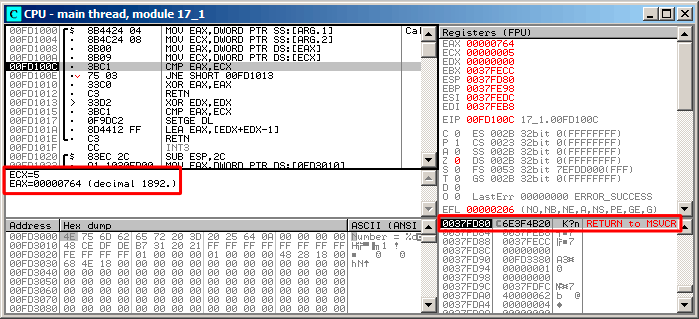
\includegraphics[scale=\FigScale]{patterns/18_pointers_to_functions/olly1.png}
\caption{\olly: \IFRU{первый вызов}{first call of} \comp}
\label{fig:qsort_olly1}
\end{figure}

\begin{figure}[H]
\centering
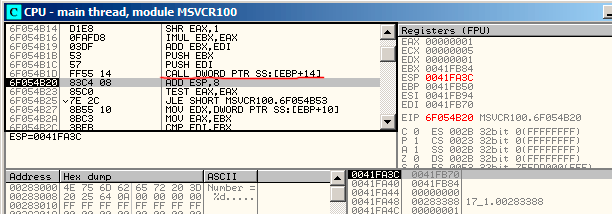
\includegraphics[scale=\FigScale]{patterns/18_pointers_to_functions/olly2.png}
\caption{\olly: \IFRU{код в}{the code in} \qsort \IFRU{сразу после вызова}{right after} \comp\EN{ call}}
\label{fig:qsort_olly2}
\end{figure}

\begin{figure}[H]
\centering
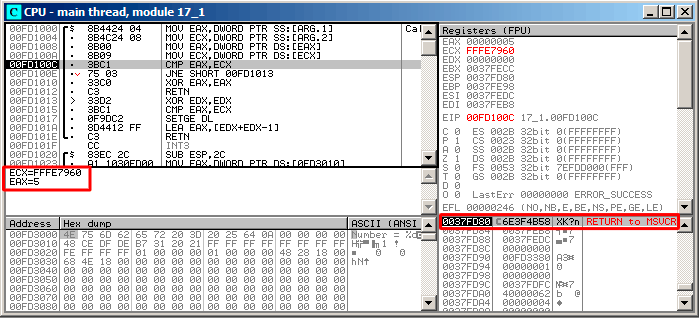
\includegraphics[scale=\FigScale]{patterns/18_pointers_to_functions/olly3.png}
\caption{\olly: \IFRU{второй вызов}{second call of} \comp}
\label{fig:qsort_olly3}
\end{figure}

\subsection{MSVC + tracer}
\index{tracer}

\IFRU{Посмотрим, какие пары сравниваются}{Let's also see, which pairs are compared}.
\IFRU{Эти 10 чисел будут сортироваться}{These 10 numbers are being sorted}: 
1892, 45, 200, -98, 4087, 5, -12345, 1087, 88, -100000.

\IFRU{Я нашел адрес первой инструкции}{I found the address of the first} \CMP 
\IFRU{в}{instruction in} \comp, \IFRU{и это}{it is} \TT{0x0040100C} 
\IFRU{и я ставлю брякпойнт на нем}{and I'm setting breakpoint on it}:

\begin{lstlisting}
tracer.exe -l:17_1.exe bpx=17_1.exe!0x0040100C
\end{lstlisting}

\IFRU{Получаю информацию о регистрах на брякпойнте}
{I'm getting information about registers at breakpoint}:

\begin{lstlisting}
PID=4336|New process 17_1.exe
(0) 17_1.exe!0x40100c
EAX=0x00000764 EBX=0x0051f7c8 ECX=0x00000005 EDX=0x00000000
ESI=0x0051f7d8 EDI=0x0051f7b4 EBP=0x0051f794 ESP=0x0051f67c
EIP=0x0028100c
FLAGS=IF
(0) 17_1.exe!0x40100c
EAX=0x00000005 EBX=0x0051f7c8 ECX=0xfffe7960 EDX=0x00000000
ESI=0x0051f7d8 EDI=0x0051f7b4 EBP=0x0051f794 ESP=0x0051f67c
EIP=0x0028100c
FLAGS=PF ZF IF
(0) 17_1.exe!0x40100c
EAX=0x00000764 EBX=0x0051f7c8 ECX=0x00000005 EDX=0x00000000
ESI=0x0051f7d8 EDI=0x0051f7b4 EBP=0x0051f794 ESP=0x0051f67c
EIP=0x0028100c
FLAGS=CF PF ZF IF
...
\end{lstlisting}

\IFRU{Я отфильтровал}{I filtered out} \TT{EAX} \AndENRU \TT{ECX} \IFRU{и получил}{and got}:

\begin{lstlisting}
EAX=0x00000764 ECX=0x00000005
EAX=0x00000005 ECX=0xfffe7960
EAX=0x00000764 ECX=0x00000005
EAX=0x0000002d ECX=0x00000005
EAX=0x00000058 ECX=0x00000005
EAX=0x0000043f ECX=0x00000005
EAX=0xffffcfc7 ECX=0x00000005
EAX=0x000000c8 ECX=0x00000005
EAX=0xffffff9e ECX=0x00000005
EAX=0x00000ff7 ECX=0x00000005
EAX=0x00000ff7 ECX=0x00000005
EAX=0xffffff9e ECX=0x00000005
EAX=0xffffff9e ECX=0x00000005
EAX=0xffffcfc7 ECX=0xfffe7960
EAX=0x00000005 ECX=0xffffcfc7
EAX=0xffffff9e ECX=0x00000005
EAX=0xffffcfc7 ECX=0xfffe7960
EAX=0xffffff9e ECX=0xffffcfc7
EAX=0xffffcfc7 ECX=0xfffe7960
EAX=0x000000c8 ECX=0x00000ff7
EAX=0x0000002d ECX=0x00000ff7
EAX=0x0000043f ECX=0x00000ff7
EAX=0x00000058 ECX=0x00000ff7
EAX=0x00000764 ECX=0x00000ff7
EAX=0x000000c8 ECX=0x00000764
EAX=0x0000002d ECX=0x00000764
EAX=0x0000043f ECX=0x00000764
EAX=0x00000058 ECX=0x00000764
EAX=0x000000c8 ECX=0x00000058
EAX=0x0000002d ECX=0x000000c8
EAX=0x0000043f ECX=0x000000c8
EAX=0x000000c8 ECX=0x00000058
EAX=0x0000002d ECX=0x000000c8
EAX=0x0000002d ECX=0x00000058
\end{lstlisting}

\IFRU{Это}{That's} 34 \IFRU{пары}{pairs}.
\IFRU{Следовательно, алгоритму быстрой сортировки нужно 34 операции сравнения для сортировки этих
10-и чисел}{Therefore, quick sort algorithm needs 34 comparison operations for sorting these 10 numbers}.

\subsection{MSVC + tracer (code coverage)}
\index{tracer}

\IFRU{Но можно также и воспользоваться возможностью tracer накапливать все возможные состояния регистров
и показать их в \IDA}{We can also use tracer's feature to collect all possible register's values
and show them in \IDA}.

\IFRU{Трассируем все инструкции в ф-ции \comp}{Let's trace all instructions in \comp function}:

\begin{lstlisting}
tracer.exe -l:17_1.exe bpf=17_1.exe!0x00401000,trace:cc
\end{lstlisting}

\IFRU{Получем .idc-скрипт для загрузки в \IDA и загружаем его}
{We getting .idc-script for loading into \IDA and load it}: \figname \ref{fig:qsort_tracer_cc}.

\IFRU{Имя этой ф-ции (PtFuncCompare) дала \IDA}{\IDA gave the function name (PtFuncCompare)}
\EMDASH{}\IFRU{видимо, потому что видит что указатель на эту ф-цию передается в \qsort}{it seems,
because \IDA sees that pointer to this function is passed into \qsort}.

\IFRU{Мы видим что указатели $a$ и $b$ указывают на разные места внутри массива, 
но шаг между указателями --- 4, что логично, ведь в массиве хранятся 32-битные значения}
{We see that $a$ and $b$ pointers are points to various places in array, but step between
points is 4---indeed, 32-bit values are stored in the array}.

\IFRU{Видно что инструкции по адресам}{We see that the instructions at} \TT{0x401010} \AndENRU 
\TT{0x401012} \IFRU{никогда не исполнялись}{was never executed} 
(\IFRU{они и остались белыми}{so they leaved as white}): 
\IFRU{действительно, ф-ция}{indeed,} \comp \IFRU{никогда не возвращала 0,
потому что в массиве нет одинаковых элементов}{was never returned 0, because there no equal elements}.

\begin{figure}[H]
\centering
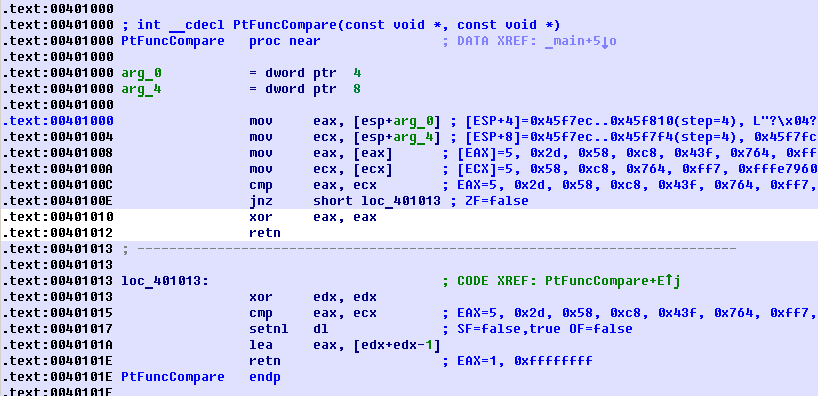
\includegraphics[scale=\FigScale]{patterns/18_pointers_to_functions/tracer_cc.png}
\caption{tracer \AndENRU IDA. N.B.: 
\IFRU{некоторые значения обрезаны справа}{some values are cutted at right}}
\label{fig:qsort_tracer_cc}
\end{figure}

\section{GCC}

\IFRU{Не слишком большая разница}{Not a big difference}:

\begin{lstlisting}[caption=GCC]
                lea     eax, [esp+40h+var_28]
                mov     [esp+40h+var_40], eax
                mov     [esp+40h+var_28], 764h
                mov     [esp+40h+var_24], 2Dh
                mov     [esp+40h+var_20], 0C8h
                mov     [esp+40h+var_1C], 0FFFFFF9Eh
                mov     [esp+40h+var_18], 0FF7h
                mov     [esp+40h+var_14], 5
                mov     [esp+40h+var_10], 0FFFFCFC7h
                mov     [esp+40h+var_C], 43Fh
                mov     [esp+40h+var_8], 58h
                mov     [esp+40h+var_4], 0FFFE7960h
                mov     [esp+40h+var_34], offset comp
                mov     [esp+40h+var_38], 4
                mov     [esp+40h+var_3C], 0Ah
                call    _qsort
\end{lstlisting}

\IFRU{Функция \comp}{\comp function}:

\begin{lstlisting}
                public comp
comp            proc near

arg_0           = dword ptr  8
arg_4           = dword ptr  0Ch

                push    ebp
                mov     ebp, esp
                mov     eax, [ebp+arg_4]
                mov     ecx, [ebp+arg_0]
                mov     edx, [eax]
                xor     eax, eax
                cmp     [ecx], edx
                jnz     short loc_8048458
                pop     ebp
                retn
loc_8048458:
                setnl   al
                movzx   eax, al
                lea     eax, [eax+eax-1]
                pop     ebp
                retn
comp            endp
\end{lstlisting}

\index{Linux!libc.so.6}
\IFRU{Реализация \qsort находится в \TT{libc.so.6}, и представляет собой просто wrapper
\footnote{понятие близкое к \gls{thunk function}} для \TT{qsort\_r()}.}
{\qsort implementation is located in the \TT{libc.so.6} and it is in fact just a wrapper
\footnote{a concept like \gls{thunk function}} for \TT{qsort\_r()}.}

\IFRU{Она, в свою очередь, вызывает \TT{quicksort()}, где есть вызовы определенной нами функции через 
переданный указатель:}
{It will call then \TT{quicksort()}, where our defined function will be called via passed pointer:}


\begin{lstlisting}[caption=
(\IFRU{файл libc.so.6, версия glibc}{file libc.so.6, glibc version}\EMDASH{}2.10.1)]

.text:0002DDF6                 mov     edx, [ebp+arg_10]
.text:0002DDF9                 mov     [esp+4], esi
.text:0002DDFD                 mov     [esp], edi
.text:0002DE00                 mov     [esp+8], edx
.text:0002DE04                 call    [ebp+arg_C]
...
\end{lstlisting}

\subsection{GCC + GDB (\IFRU{с исходными кодами}{with source code})}
\index{GDB}

\IFRU{Очевидно, у нас есть исходный код нашего примера на Си (\ref{qsort_c_src}), 
так что мы можем установить брякпойнт (\TT{b}) на
номере строки}{Obviously, we have a C-source code of our example (\ref{qsort_c_src}), 
so we can set breakpoint (\TT{b}) on line number}
(\IFRU{11-й --- это номер строки где происходит первое сравнение}{11th---the line where 
first comparison is occurred}).
\IFRU{Нам также нужно скомпилировать наш пример с ключом \TT{-g}, чтобы в исполняемом файле была
полная отладочная информация}{We also need to compile example with debugging information 
included (\TT{-g}), so the table
with addresses and corresponding line numbers is present}.
\IFRU{Мы можем так же выводить значения используя имена переменных}
{We can also print values by variable name} (\TT{p}):
\IFRU{отладочная информация также содержит информацию о том, в каком регистре и/или элементе локального
стека находится какая переменная}{debugging information also has information about which register and/or 
local stack element contain which variable}.

\index{Glibc}
\IFRU{Мы можем также увидеть стек}{We can also see stack} (\TT{bt}) 
\IFRU{и обнаружить что в Glibc используется какая-то вспомогательная ф-ция с именем}
{and find out that there are some intermediate function} 
\TT{msort\_with\_tmp()}\EN{ used in Glibc}.

\lstinputlisting[caption=GDB\IFRU{-сессия}{ session}]{patterns/18_pointers_to_functions/GDB_source.txt}

\subsection{GCC + GDB (\IFRU{без исходных кодов}{no source code})}
\index{GDB}

\IFRU{Но часто никаких исходных кодов нет вообще, так что мы можем дизассемблировать ф-цию \comp}
{But often there are no source code at all, so we can disassemble \comp function} (\TT{disas}), 
\IFRU{найти самую первую инструкцию \CMP и установить брякпойнт}{find the very first
\CMP instruction and set breakpoint} (\TT{b}) \IFRU{по этому адресу}{at that address}.
\IFRU{На каждом брякпойнте мы будем видеть содержимое регистров}
{At each breakpoint, we will dump all register contents} (\TT{info registers}).
\IFRU{Информация из стека так же доступна}{Stack information is also available} (\TT{bt}), 
\IFRU{но частичная: здесь нет номеров строк для ф-ции \comp}
{but partial: there are no line number information for \comp function}.

\lstinputlisting[caption=GDB\IFRU{-сессия}{ session}]{patterns/18_pointers_to_functions/GDB_no_source.txt}

